Our goal was to construct a minimal model that is detailed enough to capture essential microscopic features of cross-linked actomyosin networks (actin filaments with asymmetric compliance, dynamic cross-links, active motors and and continuous filament turnover), but simple enough to explore, systematically, how these microscopic features control macroscopic deformation and flow. We focus on 2D networks because they capture a reasonable approximation of the quasi-2D cortical actomyosin networks that govern flow and deformation in many eukaryotic cells\cite{cellmech_flows, salbreuxbphs}, or the quasi-2D networks studied recently {\em in vitro} \cite{rheo_2D1,rheo_2D2}.




\section{Mathematical Summary of Modeling Methodology}

\subsection{Schematic Overview}
Fig. \ref{fig:model_overview} provides a schematic overview of our model's assumptions. We model each filament as an oriented elastic spring with relaxed length $l_s$. The state of a filament is defined by the positions of its endpoints $\mathbf{x_i}$ and $\mathbf{x_{i+1}}$ marking its (-) and (+) ends respectively. The index i enumerates over all endpoints of all filaments. We refer to the filament connecting endpoint i and i+1 as filament i, and we define $\mathbf{\hat{u_i}}$ to be the unit vector oriented along filament i from endpoint i to endpoint i+1.

\begin{figure}[H]
	\centering
	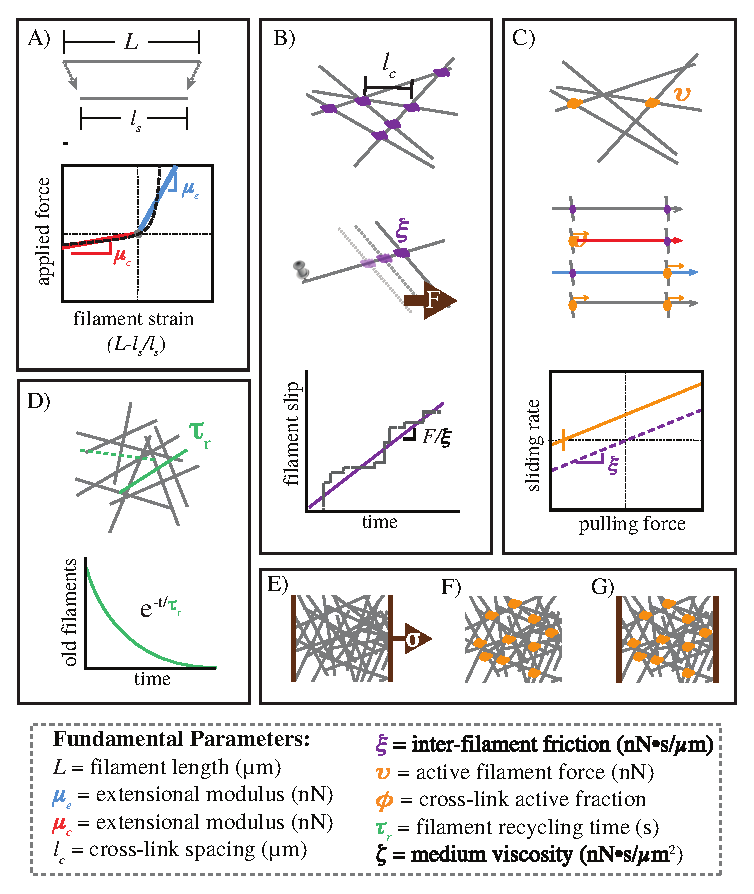
\includegraphics[width=0.8\hsize]{model/figures/Fig1}
	\caption{\label{fig:model_overview} Schematic overview of modeling framework and assumptions. \textbf{A)} Filaments are oriented linear springs that are stiffer in extension than in compression. \textbf{B)} Cross-linking occurs at all filament crossings; we represent cross link resistance as an effective drag, proportional to the relative velocity of the overlapping filaments. \textbf{C)} We represent motor activity as a linear force-velocity relationship with a fixed force at zero velocity directed towards a filament's (-) end. We implement spatial heterogeneity by imposing motor activity at a fixed fraction of filament crossover points, resulting in variation in the magnitudes of compressive vs extensile vs translational forces along individual filament segments. \textbf{D)} Whole filaments disappear at a constant rate; new filaments appear with random positions and orientations at the constant rate per unit area, such that entire network refreshes on a characteristic timescale $\tau_r$. \textbf{e-g)} Three different simulation scenarios: \textbf{E)} Passive response to uniaxial stress, \textbf{F)} Free contraction of an active network and \textbf{G)} Isometric contraction against a fixed boundary. }
\end{figure}

\subsection{Asymmetric filament compliance}
We assume (Fig. \ref{fig:model_overview}A) that local deformation of filament  i gives rise to an elastic force:

\begin{equation}
\label{eqn:spring}
\mathbf{F^{\mu}_{i,i+1}} = \mu \gamma_{i}  \mathbf{\hat{u_i}}
\end{equation}


where $ \gamma_{i} = (|\mathbf{x_{i-1}}-\mathbf{x_i}|-l_s)/l_s$ is the strain on filament i, and the elastic modulus  $\mu$ is a composite quantity that represents both filament and cross-linker compliance as in the effective medium theory of Broederz and colleagues \cite{theo_crosslinknonlinear}.  To model asymmetric filament compliance, we set $\mu = \mu_e$ if the strain is positive (extension), and $\mu = \mu_c$ if the strain is negative (compression). The total elastic force on a filament endpoint $\mathbf{i}$ can be written as:

\begin{equation}
\label{eqn:internal}
\mathbf{F^{elas}_i} =  \mathbf{F^{\mu}_{i,i+1}} - \mathbf{F^{\mu}_{i-1,i}} 
\end{equation}

In the limit of highly rigid cross-links and flexible filaments, our model approaches the pure semi-flexible filament models of \cite{theo_hlm,theo_hlm2}. In the opposite limit (nearly rigid filaments and highly flexible cross links), our model approaches that of \cite{theo_crosslinknonlinear} in small strain regimes before any nonlinear cross link stiffening. 

\subsection{Drag-like coupling between overlapping filaments}
\label{exp_drag}
Previous models represent cross-linkers as elastic connections between pairs of points on neighboring filaments that appear and disappear with either fixed or force-dependent probabilities \cite{model_taeyoon,theo_crosslinknonlinear}.  Here, we introduce a coarse-grained representation of crosslink dynamics by introducing an effective drag force that couples every pair of overlapping filaments, and which represents a molecular friction arising from the time-averaged contributions of many individual transient crosslinks (Fig. \ref{fig:model_overview}B). This coarse-grained approximation has been shown to be adequate in the case of ionic cross-linking of actin\cite{mol_fric,theo_hydroish2}, and has been used to justify simple force-velocity curves for myosin bound filaments in other contexts \cite{theo_frictionShila}. 

To implement coupling through effective drag, for any pair of overlapping filaments j and k, we write the drag force on filament j as:

\begin{equation}
\label{eqn:drag force}
\mathbf{F^{\xi}_{j,k}} = -\xi  (\mathbf{v_{j}}-\mathbf{v_{k}}) 
\end{equation}

where $\xi$ is the drag coefficient and $\mathbf{v_{j}}$, $\mathbf{v_{k}}$ are the average velocities of filaments j and k. We apportion this drag force to the two endpoints ( j, j+1) of filament j as follows: If $\mathbf{x_{j,k}}$ is the position of the filament overlap, then we assign $(1 - \mathbf{\lambda_{j,k}}) \mathbf{F^{\xi}_{j,k}}$ to endpoint j and $\mathbf{\lambda_{j,k}} \mathbf{F^{\xi}_{j,k}}$ to endpoint j+1, where $\mathbf{\lambda_{j,k}} = |\mathbf{x_{j,k}}-\mathbf{x_j}|/|\mathbf{x_{j+1}}-\mathbf{x_j}|$.

The total crosslink coupling force on endpoint i due to overlaps along filament i and i-1 can then be written:

\begin{equation}
\label{eqn: total drag couple}
\mathbf{F^{xl}_{i}} = \sum_j (1 - \mathbf{\lambda_{i,j}}) \mathbf{F^{\xi}_{i,j}} + \sum_k \mathbf{\lambda_{i-1,k}} \mathbf{F^{\xi}_{i-1,k}}
\end{equation}

where the sums are taken over all filaments j and k that overlap with filaments i and i-1 respectively.  

This model assumes a linear relation between the drag force and the velocity difference between attached filaments.   Although non-linearities can arise through force dependent detachment kinetics and/or non-linear force extension of cross-links, we assume here that these non-linear effects are of second or higher order. 

\subsection{Active coupling for motor driven filament interactions}

To add motor activity at the point of overlap between two filaments j and k ; for each filament in the pair, we impose an additional force of magnitude $\upsilon$, directed towards its (-) end (Fig. \ref{fig:model_overview}C):

\begin{equation}
\label{eqn:directedmotorforce}
\mathbf{F^{\upsilon}_{i}}=-\upsilon \mathbf{\hat{u_i}}
\end{equation}

and we impose an equal and opposite force on its overlapping partner.  We distribute these forces to filament endpoints as described above for crosslink coupling forces.  Thus, the total force on endpoint i due to motor activity can be written as:

\begin{equation}
\label{eqn:active}
\mathbf{F^{motor}_{i}} = \upsilon \sum_j (1 - \mathbf{\lambda_{i,j}}) \left (\mathbf{\hat{u_{i}}} - \mathbf{\hat{u_j}} \right ) q_{i,j}
+  \upsilon \sum_k (\mathbf{\lambda_{i-1,k}}) \left (\mathbf{\hat{u_{i-1}}} - \mathbf{\hat{u_k}} \right ) q_{i-1,k} 
\end{equation}


where j and k enumerate over all filaments that overlap with filaments i and i-1 respectively, and $q_{j,k}$ equals 0 or 1 depending on whether there is an ``active'' motor at this location. To model dispersion of motor activity, we set $q_{i,j}=1$  on a randomly selected subset of filament overlaps, such that $\bar{q}=\phi$, where $\bar{q}$ indicates the mean of $q$ (Fig. \ref{fig:model_overview}C).

\subsection{Equations of motion}

To write the full equation of motion for a network of actively and passively coupled elastic filaments, we assume the low Reynold's number limit in which inertial forces can be neglected, and we equate the sum of all forces acting on each filament endpoint to zero to obtain:

\begin{equation}
\label{eqn:syst3}
0=-l_s\zeta\mathbf{ v_i} -\mathbf{F^{xl}_i}+ \mathbf{F^{elas}_i}+\mathbf{F^{motor}_i} 
\end{equation}

where the first term represents the hydrodynamic drag on the half-filament adjoining endpoint i with respect to motion against the surrounding fluid, and $\zeta$ is the drag coefficient.

\subsection{2D network formation}

We used a mikado model approach \cite{Unterberger2014} to initialize a minimal network of overlapping unstressed linear filaments in a rectangular 2D domain. We generate individual filaments by laying down straight lines, of length L, with random position and orientation. We define the density using the average distance between cross-links along a filament, $l_c$. A simple geometrical argument can then be used to derive the number of filaments filling a domain as a function of $L$ and $l_c$ \cite{theo_hlm}.  Here, we use the approximation that the number of filaments needed to tile a rectangular domain of size $D_x \times D_y$  is $2D_xD_y/Ll_c$, and that the length density is therefore simply, $2/l_c$. 

\subsection{Modeling filament turnover}

In living cells, actin filament assembly is governed by multiple factors that control filament nucleation, branching and elongation. Likewise filament disassembly is governed by multiple factors that promote filament severing and monomer dissociation at filament ends. Here, we implement a very simple model for filament turnover in which entire filaments appear with a fixed rate per unit area, $k_{app}$ and disappear at a rate $k_{diss}\rho$, where $\rho$ is a filament density (Fig. \ref{fig:model_overview}D). With this assumption, in the absence of network deformation, the density of filaments will equilibrate to a steady state density, $k_{app}/k_{diss}$, with time constant $\tau_r = 1/k_{diss}$.   In deforming networks, the density will be set by a competition between strain thinning ($\gamma>0$) or thickening ($\gamma<0$), and density equilibration via turnover. To implement this model, at fixed time intervals $\tau_s < 0.01\cdot\tau_r$ (i.e. 1\% of the equilibration time), we selected a fraction, $\tau_s/\tau_r$, of existing filaments (i.e. less than 1\% of the total filaments) for degradation. We then generated a fixed number of new unstrained filaments $k_{app}\tau_sD_xD_y$ at random positions and orientations within the original domain.   We refer to $k_{diss}=1/\tau_r$ as the turnover rate, and to $\tau_r$ as the turnover time.


\subsection{Simulation methods}

Further details regarding our simulation approach and references to our code can be found in the Supplementary Information (\nameref{S1_Text} A.1). Briefly, equations 1-7 define a coupled system of ordinary differential equations that can be written in the form:

\begin{equation}
\mathbf{A \cdot \dot x} = \mathbf{f(x)}
\end{equation}

where $\mathbf{x}$ is a vector of filament endpoint positions, $\mathbf{\dot{x}}$ the endpoint velocities, $\mathbf{A }$ is a matrix with constant coefficients that represent crosslink coupling forces between overlapping filaments, and $\mathbf{f(x)}$ represents the active (motor) and elastic forces on filament endpoints. We smoothed all filament interactions, force fields, and constraints linearly over small regions such that the equations contained no sharp discontinuities. We numerically integrate this system of equations to find the time evolution of the positions of all filament endpoints. We generate a network of filaments with random positions and orientations as described above within a domain of size $D_x$ by $D_y$.  For all simulations, we imposed periodic boundaries in the y-dimension. To impose an extensional stress, we constrained all filament endpoints within a fixed distance $0.05\cdot D_x$ from the left edge of the domain to be non-moving, then we imposed a rightwards force on all endpoints within a distance $0.05\cdot D_x$ from the right edge of the domain.   To simulate free contraction, we removed all constraints at domain boundaries; to assess buildup and maintenance of contractile stress under isometric conditions, we used periodic boundary conditions in both $x$ and $y$ dimensions.

We measured the local velocity of the network at different positions along the axis of deformation as the mean velocity of all filaments intersecting that position; we measured the internal network stress at each axial position by summing the axial component of the tensions on all filaments intersecting that position, and dividing by network height; finally, we measured network strain rate as the average of all filament velocities divided by their positions.

We assigned biological plausible reference values for all parameters (See Table \ref{table:para}).  For individual analyses, we sampled the ranges of parameter values around these reference values shown in \nameref{S1_Table}.

\begin{table}[h]
	\centering
	\caption{Simulation parameters with reference values}
	\label{table:para}
	\begin{tabular}{|c|c|c|c|c|}
		\hline
		{\bf Parameter}             & {\bf Symbol} & {\bf Reference Value}          \\ \hline
		extensional modulus         & $\mu_e$        & $1 nN $                                               \\
		compressional modulus             & $\mu_c$     & $ 0.01 nN $                           \\
		cross-link drag coefficient & $\xi$      & $unknown $              \\
		solvent drag coefficient     & $\zeta$        & $0.0005 \frac{nN s}{\mu m^2} $      \\
		filament length             & L            & $5 \mu m$                                          \\
		cross-link spacing          & $l_c$        & $0.5 \mu m$                                         \\
		active filament force          & $\upsilon$        & $0.1 nN$                                         \\
		active cross-link fraction          & $\phi$        & $0.1<0.9$                                         \\
		domain size                 & $D_x\times D_y$            & $20\times 50 \mu m$                                 \\ \hline
	\end{tabular}
\end{table}